\documentclass[12pt,a4paper]{report}
%\renewcommand{\baselinestretch}{1.5}
%-------------------------------------------------------------------------
%
% Packages
%
%-------------------------------------------------------------------------

\usepackage{geometry}
\usepackage{setspace}
\usepackage{anyfontsize}
\usepackage{graphicx}
\usepackage{xcolor}
\usepackage{booktabs}
\usepackage{pgfplots}
\usepackage{xeCJK}
\setmainfont[Ligatures={Common,TeX}, Numbers={OldStyle}]{Times New Roman}
%\setCJKmainfont{DFKai-SB}
\setCJKmainfont{BiauKai}

% 個人設定和數據
% Google 的一些顏色
\definecolor{googleblue}{HTML}{3366CC}
\definecolor{googlered}{HTML}{DC3912}
\definecolor{googleorange}{HTML}{FF9900}
\definecolor{googlegreen}{HTML}{109618}
\definecolor{googlepurple}{HTML}{990099}

% 數據
\newcommand{\expACC}{98.2}

%-------------------------------------------------------------------------
%
% Documents
%
%-------------------------------------------------------------------------

\begin{document}

% 封面格式
\newgeometry{left=0cm,top=4cm,right=0cm,bottom=3cm}
\onehalfspacing

% 封面
\begin{titlepage}
  \begin{center}

    {\fontsize{18}{27}\selectfont
    國立臺灣大學電機資訊學院電子工程學研究所\\
    碩士論文\\
    }

    % 加點空間
    \small{~}\\

    {\fontsize{14}{21}\selectfont
    Graduate Institute of Electronic Engineering\\
    College of Engineering and Computer Science\\
    }

    {\fontsize{16}{24}\selectfont
    National Taiwan University\\
    Master Thesis\\
    }

    {\fontsize{18}{27}\selectfont
    % 加點空間
    ~\\
    ~\\

    支援Xilinx AXI DMA的Linux UIO 驅動程式\\
    Linux UIO driver for Xilinx AXI DMA\\

    % 加點空間
    ~\\
    ~\\

    劉宇唐\\
    Yu-Tang Liu\\

    % 加點空間
    ~\\

    指導教授:鄭振牟~博士\\
    Advisor: Chen-Mou Cheng, Ph.D.\\

    % 加點空間
    ~\\

    中華民國 107 年 7 月\\
    July 2018\\
    }

  \end{center}
\end{titlepage}


% 內文格式
\newgeometry{left=3cm,top=3cm,right=3cm,bottom=2cm}
\doublespacing

% 中英文摘要
%\begin{page}

\begin{center}
\large{摘要}
\end{center}

近年來,由於AI、VR產業的崛起,FPGA產業越來越受到重視。為了簡化FPGA的開發流程,使用嵌入式Linux會是一個不錯的方法。透過Linux Kernel提供的UIO驅動程式,我們可以把我們在硬體端設計出來的IP視為一個外部裝置,然後在Linux使用者空間裡的程式中,輕鬆地開發軟體端的應用。然而,有些硬體端的設計,卻無法透過同樣的方法,利用UIO驅動程式,建立裝置節點,而帶有直接記憶體存取IP的設計就是其中之一。由於UIO驅動程式並無法支援此種設計,我們必須擁有"root"	權限,才能使用我們的設計,但是提供"root"給一般使用者並不是一個好方法。在此論文中,我們修改了Linux內建的UIO驅動程式,使得一般用戶也能在使用者空間中使用帶有DMA的硬體設計。

\vspace*{2em}
{關鍵字:} \emph{賽靈思,直接記憶體存取,AXI,Linux UIO驅動程式}

%\end{page}
\begin{abstract}
In recent years, increasing importance has been attached to FPGAs with the development of AI,VR. To simplify the development process on FPGAs, embedded Linux on FPGAs will be a good way. With UIO driver provided in Linux Kernel, we can mount our block design, that is, custom IP(Intellectual Property) core in Vivado as a device node, and program it in Linux userspace. However, there are some designs that UIO driver cannot recognize. The design with DMA(Direct Memory Access) is one of them. With this kind of design, because UIO driver is not working, we need "root" to control our IP, and providing root privileges to users is never a good solution. In this thesis, we modify UIO driver so that users can easily use designs with DMA in user-space.   
%An abstract is a brief summary of a research article, thesis, review, conference proceeding or any in-depth analysis of a particular subject or %discipline, and is often used to help the reader quickly ascertain the paper's purpose. When used, an abstract always appears at the beginning of a manuscript or typescript, acting as the point-of-entry for any given academic paper or patent application. Abstracting and indexing services for various academic disciplines are aimed at compiling a body of literature for that particular subject.

%The terms précis or synopsis are used in some publications to refer to the same thing that other publications might call an ``abstract''. In management reports, an executive summary usually contains more information (and often more sensitive information) than the abstract does.


\vspace*{2em}
{\bf Keywords:} \emph{Xilinx, DMA, AXI, Linux UIO driver}

\end{abstract}

% 羅馬數字編號
\pagenumbering{roman}
\setcounter{page}{1}

% 目錄、圖目錄、表目錄
\tableofcontents
\listoffigures 
\listoftables
\clearpage

% 阿拉伯數字編號
\pagenumbering{arabic}
\setcounter{page}{1}

% 論文正文
\chapter{Introduction}
\label{cha:introduction}
FPGA(Field Programmable Gate Array) is special hardware device that allows people can design and verify their thoughts easily and quickly comparing to ASIC. To design hardware part in PL(Programmable Logic) side, it need to use development tools(e.g.Vivado) provided by FPGA's manufaction. It is reasonable, because how to convert HDL to the designs that FPGA can recognize depends on rules of its own provider. So hardware design facilitation is basicly in control of FPGA vendors. On the other hand, software designing should be much easier and more free, because we can use languages and libaries that we are familiar with. But in fact, we still rely on using SDK tools to design our software system instead. In tradition, we build a ``bare metal'' program to control our system, and sometimes, the program may includes some special libraries only provided in SDK. In software engineer's perspective, things should not be that complicated if we just want to do the simple things like, reading or writing datas to registers in PL side. So there come's some solutions to flexible the software development.  
%本章為簡易的LaTeX範本,使本文略微豐富些。由於編譯器是使用XeLaTeX,中英文可以無縫直接輸入,不需要額外繁瑣的環境設定。 Section~\ref{sec:simpletechnique1} 是撰寫文件時可以用的一些小技巧。 Section~\ref{sec:figandtable} 示範LaTeX繪製圖表的功能。

%-------------------------------------------------------------------------
% Section: 簡單範例和小技巧
%-------------------------------------------------------------------------

\section{Motivation}
\label{sec:Motivation}

 To simplify the develop flow, introducing embedded system on FPGA becomes more popular in recent years. In embedded Linux we can apply UIO driver to our custom IP in PL side and control it in user space application, just like it is a external device. However there are still some issues, that make UIO can not work correctly, the designs using AXI-Stream register with DMA controller is the one of them. With this design, we can only control DMA controller to transfer data ``to'' or ``from'' our custom IP, and this need ``root'' privileges. But giving ``root'' to a user that only want to control the custom IP is overkill. So we need to find out a soluion to this problem. 

%首先先示範一行簡單的數學式:
%\begin{equation} \label{eq:sample1}
%  y = \sum_{i=1}^{n}f(x_i),
%\end{equation}
%個人認為這比起用 Word 的方程式專業不少,在輸入上也方便得多。不過有些人可能會發現這條式子和一些常見的課本(像微積分)上的式子長得略微不同,這是因為他們額外安裝了付費的數學字型 MathTime Professional,約莫台幣三千元,可以讓 $y$ 和一些粗體希臘字母長得好看些,一些數學符號的間距也會被修正。

%不管是哪個科系,很多時候會需要把一些數據寫進論文裡。若是在論文撰寫的同時仍然有機會更動數據,那麼找出該數字出現的每個地方並一一改寫,這是一件很崩潰的事。所以小弟我的做法是把一些關鍵的數字寫在 \texttt{src/def.tex} 裡,利用 \texttt{newcommand} 去定義該數字。例如某項實驗做出來的準確度為 \expACC{}\%,那麼之後需要變動就只要改寫 \texttt{src/def.tex} 中的 \texttt{expACC} 即可。

%在編譯完一份文件,切莫忘記檢查 \texttt{.log} 檔案中是否含有 Overfull hbox 或 Underfull hbox 等訊息。前者代表存在一行文字無法左右貼齊,會有文字超出到頁邊空白處,後者則是在左右貼齊的過程中,文字間的留白過大。

%-------------------------------------------------------------------------
% Section: 圖表
%-------------------------------------------------------------------------

\section{Contribution}
\label{sec:contribution}
We propose a develop flow to use UIO to control DMA controller to communicate with AXI-Stream IP, with a little modified of UIO driver and specific format settings in device tree file. We rewrite \textbf{read()/write()} functions in UIO to send DMA transactions to DMA controller. The whole scenario is very simple and intuitive, and is not much different from original flow. The data transfering efficiency is also good, it reaches about 17mb/s with AXI-Stream FIFO. 
%表格當然可以用 Excel 匯出成 PDF 或圖檔在匯進來,但我是直接用 LaTeX 繪製,如 Table~\ref{tab:sample1}。圖也是一樣, Figure~\ref{fig:lena} 是一張影像處理常用的圖。但若是漂亮的數據圖繪製,那小弟我也是推薦使用 LaTeX 的向量繪圖功能。 Figure~\ref{fig:runtimeanalysis} 是用 PGFPlots 這個套件以存放在 \texttt{data/result.txt} 的實驗數據畫的圖,若是用 Matlab 畫得就比較快但比較醜。另外值得注意的是數據越多畫越久,上千個資料點可能會需要三秒到五秒不等的時間。

%\begin{table}
%\centering
%\begin{tabular}{clr|clr}
%  \toprule
%    \textbf{Id} & \textbf{Family} & \textbf{\#} & \textbf{Id} & \textbf{Family} & \textbf{\#} \\
%  \midrule
%  A & DroidKungFu   & 473 & K & FakePlayer      &  74 \\
%  B & DorDrae       & 420 & L & Wroba           &  74 \\
%  C & Meds          & 221 & M & Plankton        &  63 \\
%  D & Fakeguard     & 203 & N & DroidDreamLight &  52 \\
%  E & Boxer         & 202 & O & Cawitt          &  51 \\
%  F & Kmin          & 183 & P & Badao           &  46 \\
%  G & Rooter        & 117 & Q & Fake10086       &  46 \\
%  H & Boqx          & 114 & R & Cupi            &  39 \\
%  I & DroidAp       & 106 & S & Coogos          &  39 \\
%  J & DroidKungFu3  &  93 & T & DroidDream      &  39 \\
%  \bottomrule
%\end{tabular}


%\caption{Top 20 malware families in the dataset.}
%\label{tab:sample1}
%\end{table}

%\begin{figure}
%  \centering
%  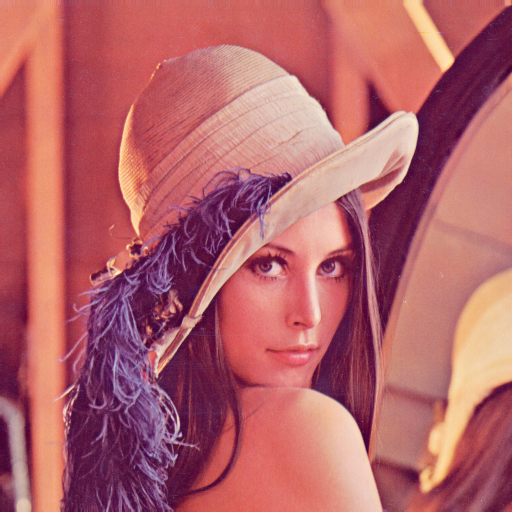
\includegraphics[scale=0.5]{images/lena.png}
%  \caption[Short caption for Lena]{Long caption for Lena.}
%  \label{fig:lena}
%\end{figure}

%\begin{figure}
%\centering
%  \begin{tikzpicture}
%    \begin{axis} [
%      xlabel={Size of classes.dex (MiB)},
%      ylabel={Time (sec)},
%      xmin=0.01,
%      xmax=144,
%      xmode=log,
%      ymin=0.01,
%      ymax=144,
%      ymode=log,
%      height=10cm,
%      width=10cm,
%      grid=major,
%      legend cell align=left,
%      legend pos=south east,
%    ]
%    
%    \addplot [color=gray,only marks,mark size=1pt] table [x=size,y=time] {data/result.txt};
%    \addplot [color=black] coordinates {(0.01,0.0471) (10,55.5648)} node[below] at (0.7, 0.7) {$O(n^{1.024})$};

%    \legend{Samples, Estimation}

%    \end{axis}
%  \end{tikzpicture}
%  \caption{Runtime analysis of Androguard.}
%  \label{fig:runtimeanalysis}
%\end{figure}

%-------------------------------------------------------------------------
% Section: 參考文獻
%-------------------------------------------------------------------------

%\section{編輯參考文獻}
%\label{sec:ref}

%LaTeX 另個方便的地方就是參考文獻,我是使用 IEEEtran 的格式,它會依照出現的次序編排。若是使用 IEEEtranS 則會以作者姓氏為依據。另外需要注意它會雞婆地把書目標題的大小寫做改動,要保持原樣就得在 \texttt{reference.bib} 的標題加括弧,像是 \cite{permissionevolution} 和 \cite{permissionevolution2} 的差別。

%-------------------------------------------------------------------------
% Section: 總結
%-------------------------------------------------------------------------

%\section{總結}
%\label{sec:summary}

%用 LaTeX 寫論文或作業很方便,但速度快慢取決於對於 LaTeX 的熟悉程度,還不熟的同學可以搜尋大家來學LaTeX \cite{latex123},以入門來說是滿不錯的,祝各位碩博士生論文順利。





%-------------------------------------------------------------------------
% Section: 前情提要
%-------------------------------------------------------------------------
\chapter{Preliminaries}
\label{cha:Preliminaries}
In this chapter, we introduce the background technology for our work. 
Embedded Linux, UIO Driver, AXI Bus, and DMA.


%-------------------------------------------------------------------------
% Section: 嵌入式理你斯
%-------------------------------------------------------------------------

\section{Embedded Linux}
\label{sec:Embedded Linux}

Embedded Linux is a kernel and set of libraries and utilitied designed to run
on an embedded system(for example:router). 

\subsection{Device Tree}
\label{subsec:Device Tree}

Device Tree is a mechanism to describe all hardware and devices of a system. In early Linux 
kernel, hardware description is hardcode in kernel file, so porting kernel to different
ARM-CPU based system is painful. To solve this problem, Devcice Tree is introduced. 
Like x86 based system, we should consider Linux kernel image is a black box, and give the 
hardware informations of system to kernel. \\
%
In FPGA development flow, the whole system keeps almost the same, the only thing changes 
is our design in PL(Programmable Logic) side. To boot Linux with different PL design, only 
a little modification of devicetree file is needed.     


\subsection{Linux Kernel Driver}
\label{subsec:Linux Kernel Driver} 


%-------------------------------------------------------------------------
% Section: UIO driver
%-------------------------------------------------------------------------

\section{UIO}
\label{sec:UIO}
For many types of devices, creating a Linux kernel driver is overkill. All that is really needed 
is some way to handle an interrupt and provide access to the memory space of the device. To address 
this situation, the userspace I/O system (UIO) was designed.Hardware that is ideally suited for an 
UIO driver fulfills all of the following:
%
\begin{itemize}
\item The device has memory that can be mapped.
\item The device can be controlled completely by writing to this memory.
\item The device usually generates interrupts.
\item The device does not fit into one of the standard kernel subsystems.
\end{itemize}
%
Figure~\ref{fig:UIO Driver} shows how the UIO system works, in software-side of FPGA development, we 
only care about the value in the hardware register and when we can get the correct value, so memeory
-mapping to user-spcae application and interrupt handler is realy enough in our design flow.  
%
\begin{figure}[!htb]
  \centering
  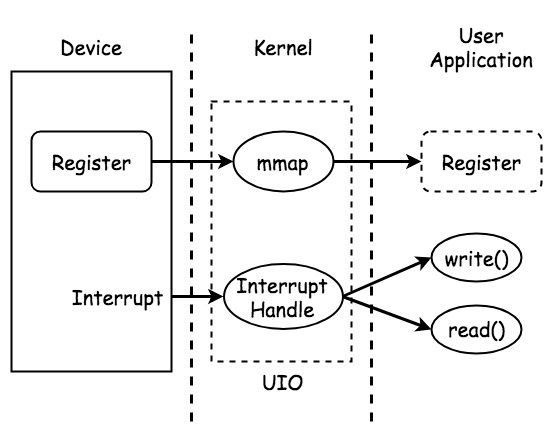
\includegraphics[scale=0.5]{images/uio.jpg}
  \caption[The UIO way.]{The UIO way.}
  \label{fig:UIO Driver}
\end{figure}

%-------------------------------------------------------------------------
% Section: AXI Bus
%-------------------------------------------------------------------------
\section{AXI Bus}
\label{sec:AXI Bus}


\subsection{AXI Stream }
\label{subsec:AXI Stream}

%-------------------------------------------------------------------------
% Section: DMA
%-------------------------------------------------------------------------
\section{DMA}
\label{sec:DMA}

\subsection{DMA Engine }
\label{subsec:DMA Engine}
%-------------------------------------------------------------------------
% Section: our main work
%-------------------------------------------------------------------------

\chapter{Proposed solution }
\label{cha:proposed solution }


\begin{figure}[!htb]
  \centering
  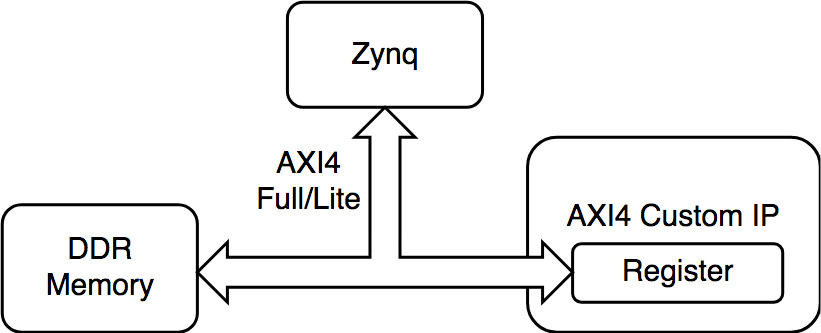
\includegraphics[scale=0.5]{images/AXI4customIP.jpg}
  \caption[Custom IP with AXI4-Lite/Full Register.]{Custom IP with AXI4-Lite/Full Register.}
  \label{fig:Custom IP with AXI4-Lite/Full Register.}
\end{figure}

%-------------------------------------------------------------------------
% Section: 
%-------------------------------------------------------------------------

\section{Linux UIO driver for AXI DMA}
\label{sec:Linux UIO driver for AXI DMA}

\subsection{Scatter Gather}
\label{subsec:Scatter Gather}
In tranditional DMA transaction, it can only accept a contiguous (nonsegmented) block of
physical memory, so, if we want to use DMA in userspace, and we can not get a contiguous 
memory space(like CMA), then we need to use DMA Scatter/Gather mode. This mode allows non-
contiguous (nonsegmented) block of physical memory and this mode need to be turn on in Vivado 
design first. In this mode, DMA controller automatically give the start address of the 
segmented of memory after the previous transaction of segmented memory is completed. To 
apply this mode, we need to construct a special data structure, Scatterlist, which collects 
start address and lengths of segmented block of user buffer memory. DMA engine will do the
transaction according to this list. 


\subsection{Cache Coherency}
\label{subsec:Cache Coherency}
While using DMA to do the data transfering, it may lead cache coherency problems. Figure~\ref{fig:Cache Coherency Problems.}
shows the cache coherency problem, both read and write may lead this problem, so if we want to 
transfer correct data, we must solve this problem.

My first trial is try to solve this problem in user application, that is, announce ``volatile'' 
buffer to prevents an optimizing compiler from optimizing away subsequent reads or writes and 
thus incorrectly reusing a stale value or omitting writes. 
\begin{figure}[!htb]
  \centering
  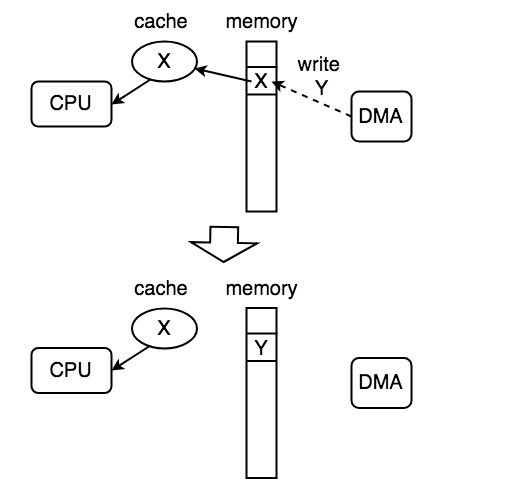
\includegraphics[scale=0.5]{images/cache_coherency.jpg}
  \caption[Cache Coherency Problems.]{Cache Coherency Problems.}
  \label{fig:Cache Coherency Problems.}
\end{figure}
%-------------------------------------------------------------------------
% Section: 圖表
%-------------------------------------------------------------------------

\section{Implementation}
\label{sec:Implementation}





%-------------------------------------------------------------------------
% Section: 總結
%-------------------------------------------------------------------------
\chapter{Environment Framework}
\label{cha:Environment Framework}

In this chapter, we introduce the device, environment and software that we used in our experiment. 
%\begin{itemize}
%\item We choose ZedBoard() as our target FGPA platform.
%\item Linux Kernel is compiled from the github repository provided by Xilinx.\cite{xlnxkernel}
%\item Linaro\cite{linarofs} is put in 2nd partition of SD card as our root file system.
%\item All our custom stream IPs are designed(and provided) in Vivado 2016.04.
%\item Device Tree files are generated by SDK 2016.04 and github repository provided by Xilinx\cite{xlnxdevicetree}
%\end{itemize}



\begin{enumerate}[label=(\roman*)]
\item We choose Xilinx ZedBoard as our target FGPA platform.
	\begin{enumerate}
	\item Dual ARM® Cortex™-A9 MPCore™
	\item 512 MB DDR3 memory (1066 Mbps)
	\end{enumerate}
\item Linux Kernel is compiled from the github repository provided by Xilinx.\cite{xlnxkernel}
	\begin{enumerate}
	\item Kernel version is 4.9.0
	\item GCC version is 5.4.0
	\end{enumerate}
\item Linaro\cite{linarofs} is put in 2nd partition of SD card as our root file system.
\item All our custom stream IPs are designed(and provided) in Vivado 2016.04.
\item Devicetree files are generated by SDK 2016.04 and github repository provided by Xilinx\cite{xlnxdevicetree}
\end{enumerate}

Although, we use some relatively old version of Xilinx deveplop software, but our contribution is basiclly out of the version problem. If the version compatible is well handled by Xilinx, our flow and code should work well directly, and if not, only little modification is needed.

\newpage
\section{Some Issues about Devicetree File}
\label{sec:Some Issues about Devicetree File}
This section we talk about some issues about devicetree file. We have mentioned devicetree file in former chapter~\ref{subsec:Device Tree}, but here we'll discuss some problems we met when we do the experiment, and it might be some bugs of devicetree compiler or devicetree generator of Xilinx SDK. Because this is not about how we solve the problem, so we separate this part here.

There may have some wrong settings if you directly use the devicetree file generated by Xilinx SDK. For example, the interrupt settings of DMA controller or our custom IP in deivcetree file may not follow the Vivado design. The interrupt number and interrupt type 
may be not the same as we expect. See the following exaple:{}

{\renewcommand\baselinestretch{0.8}\selectfont
\begin{lstlisting}[frame=single,language=C]
dma@40400000 {
	#dma-cells = <0x1>;
	clock-names = "s_axi_lite_aclk", "m_axi_sg_aclk", "m_axi_mm2s_aclk", "m_axi_s2mm_aclk";
	clocks = <&clk 0xf &clk 0xf &clk 0xf &clk 0xf>;
	compatible = "xlnx,axi-dma-1.00.a";
	interrupt-parent = <0x3>;
	interrupts = <0x0 0x1d 0x4 0x0 0x1e 0x4>;
	reg = <0x40400000 0x10000>;
	xlnx,addrwidth = <0x20>;
\end{lstlisting}
\par}

In ``interrupt'' property,	``interrupts = <0x0 0x1d 0x4 0x0 0x1e 0x4>;'' means we have two interrupts, <0x0 0x1d 0x4> and <0x0 0x1e 0x4> because we have two DMA channel in our design. The second term(0x1d and 0x1e) is the interrupt number and should be determined when we connect DMA controller to the CPU in Vivado design. But in fact, the generated devicetree file sometimes may set wrong number to this term, and  cause the driver can not probe the device correctly. The third terms(in our example, both are 0x4) is the interrupt type, this term is related to how we treat the interrupt signal, because the devicetree compiler can't know how we design, it just put a default value to this term. So make sure that the setting in devicetree file is corresponding with the design. The interrupt type definition is in \cite{intterrupttypes}

Some label problem may happen also. In devicetree, we can define labels for convenience, let's take alook at the above example again, note that, in ``clocks'' property, it uses label ``\&clk'', to get the correct clock, so there must have some settings like:

{\renewcommand\baselinestretch{0.8}\selectfont
\begin{lstlisting}[frame=single,language=C]
clk: clkc@100 {
	#clock-cells = <0x1>;
	compatible = "xlnx,ps7-clkc";
	fclk-enable = <0xf>;
	clock-output-names = "armpll", "ddrpll", "iopll", "cpu_6or4x", "cpu_3or2x", "cpu_2x", "cpu_1x", "ddr2x", "ddr3x", "dci", "lqspi", "smc", "pcap", "gem0", "gem1", "fclk0", "fclk1", "fclk2", "fclk3", "can0", "can1", "sdio0", "sdio1", "uart0", "uart1", "spi0", "spi1", "dma", "usb0_aper", "usb1_aper", "gem0_aper", "gem1_aper", "sdio0_aper", "sdio1_aper", "spi0_aper", "spi1_aper", "can0_aper", "can1_aper", "i2c0_aper", "i2c1_aper", "uart0_aper", "uart1_aper", "gpio_aper", "lqspi_aper", "smc_aper", "swdt", "dbg_trc", "dbg_apb";
	reg = <0x100 0x100>;
	ps-clk-frequency = <0x1fca055>;
	linux,phandle = <0x1>;
	phandle = <0x1>;
};
\end{lstlisting}
\par}

But in the devicetree file generated by SDK, it sometimes use the label without pre-set the label, using the above example, it uses ``\&clk'' in ``dma'' node, but it does not set ``clk'' label to ``clkc'' node. So if there are some error messages about the reference when generating the devicetree file, make sure the above problems is solved.

%-------------------------------------------------------------------------
% Section: 簡單範例和小技巧
%-------------------------------------------------------------------------





%-------------------------------------------------------------------------
% Section: 分析
%-------------------------------------------------------------------------
\chapter{Analysis}
\label{cha:Analysis}

%-------------------------------------------------------------------------
% Section: FIFO
%-------------------------------------------------------------------------

\section{FIFO}
\label{sec:FIFO}

%-------------------------------------------------------------------------
% Section: Stream IP
%-------------------------------------------------------------------------

\section{Stream IP}
\label{sec:Stream IP}

%-------------------------------------------------------------------------
% Section: 比較
%-------------------------------------------------------------------------
\section{Comparison}
\label{sec:Comparison}







%-------------------------------------------------------------------------
% Section: 總結
%-------------------------------------------------------------------------
\chapter{Conclusion and Future Works}
\label{cha:conclusion and Future Works}

In this thesis, we design a flow and modify the UIO driver so that we can control our custom AXI4-Stream IP in Linux on FPGA easily. The driver efficiency is also satisfactory, and our modification is also little, we even provide a script file to run all things, if set properly. The final goal of our works is that our modified UIO driver can be merged into Linux kernel. Rather than write a whole new driver, we think that most FPGA developers use UIO driver to communicate with their own IP, so make UIO driver ``better'' is a ``better'' way to solve the problem that we have no useful driver to help us control the AXI4-Stream IP. In conclusion, we think our work is useful for people who want to develop an application on FPGA

In future, there are still some works can be done, for example, Xilinx has other DMA components provided in Vivado that is, AXI VDMA and AXI CDMA. VDMA is a special DMA used for video purpose, and CDMA is a memory-mapped to memory mapped DMA, like FIFO with AXI DMA. We are not very sure whether the usage of these components is as same as AXI DMA, this needs more test and research. 






% 參考文獻
\clearpage
\addcontentsline{toc}{chapter}{References}
\renewcommand{\bibname}{References}
\bibliographystyle{IEEEtran}
\bibliography{IEEEabrv,reference}

\end{document}